% Condensed report: main body targeted at <= 8 A4 pages; supporting detail in appendices.
% Compile twice with pdfLaTeX. Put optional figures in ./images/.
\documentclass[10pt,a4paper]{article}
\usepackage[a4paper,margin=0.82in]{geometry}
\usepackage{booktabs,amsmath,array,tabularx,graphicx,caption,placeins,tikz}
\usetikzlibrary{arrows.meta,positioning}
\usepackage[hidelinks]{hyperref}
\graphicspath{{images/}}
\setlength{\emergencystretch}{2em}
\setlength{\parskip}{3pt}
\setlength{\parindent}{0pt}
\captionsetup{font=small,skip=3pt}
\renewcommand{\arraystretch}{1.06}
\newcommand{\safeimage}[2][]{\IfFileExists{images/#2}{\includegraphics[#1]{#2}}{\fbox{\parbox{0.75\linewidth}{\centering Figure file: \texttt{\detokenize{#2}}\\(add to images/ to display)}}}}
\title{Predicting HDB Monthly Rent: Feature Engineering and Model Comparison}
\author{Gold Miner (Group 12)}
\date{November 2026}
\begin{document}
\maketitle
\begin{abstract}
We predict Singapore HDB monthly rent from 150,000 labelled transactions (January 2021--March 2025), and generate predictions for 50,000 unlabelled competition records. We compare core CatBoost, auxiliary-feature CatBoost, a town-specific multistage architecture, and a global CatBoost with a property-adjusted rental time index. The strongest contributions are chronological evaluation, careful address and MRT features, and temporal or historical-rent modelling. The best reported competition RMSE is \textbf{432.50} (\texttt{add\_mrt}); the latest separate submission scores 441.46. Distinct hold-out windows are reported separately rather than ranked as though directly comparable.
\end{abstract}

\section{Problem and evaluation protocol}\label{sec:intro}
The target $y$ is monthly rent (SGD). The original labelled and unlabelled files have ten common input fields and no missing cells; the labelled set has 150,000 rows and the unlabelled set 50,000. Labelled approvals span January 2021--March 2025. Unlabelled approvals span March 2025--July 2026, including an overlapping calendar month but no known competition labels. The goal is forward prediction, so random splits alone are not an adequate performance estimate.

\begin{table}[htbp]\centering\small
\caption{Evaluation windows. These names are deliberately kept distinct.}\label{tab:splits}
\begin{tabularx}{\linewidth}{@{}p{0.28\linewidth}X@{}}\toprule
Experiment & Fit / scoring period \\\midrule
Multistage training / validation / test & Fit through Sep 2024; validate Oct--Dec 2024; test Jan--Mar 2025. Validation alone selects the epoch.\\
Core six-month hold-out & Fit through Sep 2024; score Oct 2024--Mar 2025 (17,198 rows).\\
Auxiliary development / assessment & Three expanding six-month development folds through Oct 2023; separate 17-month assessment fits through Oct 2023 and scores Nov 2023--Mar 2025.\\
Global CatBoost Search / Confirm & Fit through Sep 2024; Search Oct--Dec 2024; Confirm Jan--Mar 2025. Confirm was inspected during iteration and is \emph{not} an untouched test.\\
Competition & 50,000 unlabelled predictions evaluated by the competition platform; not directly comparable to local splits.\\
\bottomrule\end{tabularx}\end{table}


\subsection*{Metric and scope}
We report root-mean-square error in the target unit, SGD per monthly lease:
\begin{equation}\label{eq:rmse} \mathrm{RMSE}=\sqrt{\frac{1}{N}\sum_{i=1}^{N}(y_i-\hat y_i)^2}.\end{equation}
RMSE penalizes large rental errors and therefore emphasizes atypical high-rent transactions as well as systematic market-level bias. It is computed on the rows belonging to each named scoring window. The private competition labels are not available in the supplied data: their score is a platform-reported result, not a locally recomputed validation metric. Model selection therefore must not rely on treating a competition score as a substitute for chronological validation.

For the multistage experiment, months through September 2024 train parameters, October--December 2024 choose the fitted model, and January--March 2025 are reserved for final local testing. The six-month CatBoost hold-out scores those last two periods together, while the auxiliary experiment intentionally uses a much earlier fit cutoff. These choices answer different questions: near-term prediction, robustness to an extended future period, and architecture selection. We preserve the differences rather than presenting the smallest number as evidence of a universal winner.


\section{Data processing and feature selection}\label{sec:process}
\textbf{Core data.} We consistently normalize town, street, block, flat type, flat model, and furnishing strings (case, spaces and room-type notation), parse dates and create an approval-month index $12(\mathrm{year}-2021)+(\mathrm{month}-1)$. We construct a building key from \emph{block + street}, compute lease age at approval, and flag the one impossible lease-age record rather than deleting it. Duplicate rows and unusual rents are retained because repeated predictors can correspond to distinct transactions. Furnished status and the upfront fee are constant and removed from the core baseline. Unseen buildings in the competition file are accommodated by the categorical encoder.

\textbf{Spatial and external information.} The block/address join supplies coordinates, completion year and maximum building floor; derived features include building age, distance to the CBD, nearby block density, and proximity to MRT, schools and malls. We distinguish existing open MRT stations from planned stations when constructing accessibility features, although the available snapshot lacks opening dates. Macro candidates include lagged COE premiums and stock-market measures; their temporal alignment is constrained to observations available before the rental month. The rebuilt candidate audit explores substantially more columns than are fitted in any one model; the separate multistage input ledger has 94 auxiliary columns. Detailed family inventories, source limitations and EDA figures are in Appendices~\ref{app:eda}--\ref{app:aux}.

\textbf{Historical rental information and leakage control.} Group-mean encodings use only previously labelled rents, with smoothing and time-window rules; no scored-month labels may enter a fitted encoding. A three-month mean can be written
\begin{equation}\label{eq:shrinkmain}m_g=\frac{n\bar r_g+20\bar r}{n+20},\end{equation}
where $\bar r_g$ and $\bar r$ are the group and island-wide means in earlier eligible months. For future dates beyond available labels, such statistics may become sparse or unavailable; we therefore assess history features separately rather than treating them as guaranteed future information. All estimated imputers, encoders, scalers and models are fitted within each experiment's training period. The full list of EDA variables and unused auxiliary features is deferred to the appendices.


\subsection{Practical feature construction pipeline}
After the deterministic cleaning, features are joined by a normalized block--street building key rather than by block number alone. This retains a one-to-one rental-row mapping when one block number is reused on different roads. The address lookup matches all labelled and unlabelled rows and preserves their original order, a requirement for submission alignment. Latitude and longitude supply great-circle distances to facilities using Earth radius 6,371 km; completion year and lease commencement year yield different building-age and lease-age measures. Neither building maximum floor nor geographic block density is a substitute for the unavailable level of the individual rental unit.

\begin{table}[htbp]\centering\small
\caption{Core modelling features, their transformations and use.}\label{tab:featurepipeline}
\begin{tabularx}{\linewidth}{@{}p{0.23\linewidth}X p{0.22\linewidth}@{}}\toprule
Feature family & Construction & Main role\\\midrule
Dwelling & Flat type/model, area, age of lease at approval & Strong baseline predictors\\
Address & Normalized town, street, block and joint building key & Categorical geographic detail\\
Time & Approval year, month and monotonic month index & Market progression\\
Building and region & Geocoded block; age, central distance, nearby density & Location refinement\\
Transport & Nearest open MRT, line and radius counts; planned separately & Selected auxiliary gain\\
Macro/history & Completed-month COE/stock values; prior labelled-rent group means & Separate timed experiments\\\bottomrule
\end{tabularx}\end{table}

\subsection{Selection and temporal availability}
We do not assume that every engineered field helps. The core baseline establishes the effect of adding dwelling and address information; Model~2 then applies locked feature-family comparisons. In particular, the rebuilt auxiliary audit is a candidate inventory rather than an instruction to fit all 1,878 conceptual columns. Individual-stock and adjusted-price candidates are kept in a monthly panel instead of repeated as though they were independent flat-level records. Scalers and derived statistics that learn from a distribution are fitted to the training period of the corresponding experiment, not to future labels.

The time of information availability differs across feature families. Geometry and historical block metadata can be attached from their snapshot, though this is not proof that their historical state was identical. Market variables for month $T$ use observations from $T-1$ or earlier. Recent-rent encodings use the preceding three available labelled months and shrink group means toward the contemporaneous island-wide mean by Equation~\eqref{eq:shrinkmain}. The same-month rent is excluded. When predicting far beyond March 2025, the recent-labelled window is not continuously refreshed; this makes the future deployment of history-dependent models a meaningful limitation, not merely a missing-value detail.


\section{Models and experimental results}\label{sec:models}
\subsection{Model 1: Core CatBoost baseline}\label{sec:m1}
A CatBoost regressor learns nonlinear interactions between town, flat type, location, area, age and approval time; the fixed initial configuration uses 600 iterations, learning rate 0.05 and depth 8. Chronological nested-mean baselines establish how much information each feature set adds. The six-month hold-out shows a substantial reduction in RMSE from \textbf{795.76} for a global mean to \textbf{454.29} for CatBoost (Table~\ref{tab:coremain}). The tree's largest reported feature importances are flat type (28.04), month index (22.62), and town (16.69). The mean prediction error on this hold-out is $-36.29$ SGD, indicating underprediction of later rents; full monthly, flat-type and rolling-fold diagnostics are deferred to Appendix~\ref{app:coremodels}.
\begin{table}[htbp]\centering\small
\caption{Core baseline on the Oct 2024--Mar 2025 six-month hold-out; monthly-rent RMSE (SGD).}\label{tab:coremain}
\begin{tabular}{lr}\toprule Model & RMSE\\\midrule
Global mean & 795.76\\Town mean & 778.62\\Town + flat-type mean & 565.58\\CatBoost & \textbf{454.29}\\\bottomrule\end{tabular}\end{table}


\paragraph{Baseline robustness across time.}
The fixed core CatBoost was also evaluated on three expanding April--March yearly folds. RMSE declines from 719.52 (April 2022--March 2023) to 599.59 (April 2023--March 2024) and 477.47 (April 2024--March 2025). Corresponding mean errors are $-370.41$, $-146.57$, and $-35.74$ SGD (prediction minus observation). This indicates that a model fitted on the earliest months badly underestimates a later rental market; larger and more recent fitting windows improve calibration. These are not the multistage validation/test scores.

A random hold-out of the same size yields RMSE 476.25 versus 454.29 for the chronological six-month hold-out, but lower bias ($-6.64$ rather than $-36.29$ SGD). The reason to prefer chronological assessment is its alignment with deployment, not an expectation that it always gives the larger error. Month-wise, the later hold-out maintains negative mean error, increasing in magnitude to $-53.33$ SGD in March 2025. Executive flats show a higher RMSE (537.59) than 3-room flats (426.74), suggesting that rent levels and uncommon dwelling combinations remain challenging. Detailed fold tables and error-by-type counts are retained in Appendix~\ref{app:coremodels}.

\subsubsection{Global CatBoost with a Rental Time Index}
\label{sec:time-index}

\textbf{Motivation}

Model~4 extends Model~1's global CatBoost approach with selected
auxiliary inputs, complete-address categorical encoding, and an
explicit rental time index.
It investigates whether separating market-level temporal movement
from property-level rent prediction improves forecasting while
preserving the original rent labels and chronological split.

The regional residual pipeline provides a separate local control
during this experimental series.
Early trials involving floor area, building age, and historical-rent
features produced limited or inconsistent gains.
A global direct-rent CatBoost instead pools observations across towns,
allowing one model to learn shared relationships between dwelling
attributes, location, and monthly rent.

Temporal extrapolation remains a separate problem.
The competition file extends to July 2026, 22 months beyond the
September 2024 fitting cutoff.
A tree can split on an observed approval-month index, but that
feature alone does not extrapolate a continuing trend beyond the
fitting range.
Model~4 therefore estimates a property-adjusted rental time index
separately from the conditional rent model.

\textbf{Structure}

The fitting period is January 2021--September 2024
(132{,}802 rows).
Search is October--December 2024 (8{,}274 rows), and Confirm is
January--March 2025 (8{,}924 rows).
These boundaries match Model~3's training, validation, and test
periods, respectively.
The separate names identify this iterative experimental series.
Original rents, row membership, and row order remain unchanged.

Search controls early stopping and eligibility for Confirm evaluation.
Confirm results also informed subsequent decisions about which
configurations to retain.
Confirm is therefore treated as an additional validation period
rather than an independent test set.

The final model uses 26 inputs: 17 numeric and nine categorical
columns.
Numeric inputs describe floor area, building and lease age,
completion and lease commencement years, maximum floor,
flat-type and flat-model ranks, the approval-month index,
coordinates, and amenity distances.
The constant-zero fee is also retained.
Categorical inputs identify town, block, street, flat model,
the nearest amenities, and the complete address.
The complete-address category concatenates normalized town,
street, and block without using rent labels.
Numeric missing values use fitting-period medians, with no
numerical scaling.
Categories use CatBoost's native categorical processing and the
saved missing-category fallback.

Only fitting-period rents estimate the time index.
Observable property groups are defined by town, street, block,
flat type, flat model, and floor area.
Groups observed in at least two distinct fitting months identify
the fixed-effects model
\begin{equation}
\label{eq:model4-fixed-effects}
\log y_i
=
\alpha_{g(i)} + b_{t(i)} + \epsilon_i,
\end{equation}
where $\alpha_{g(i)}$ is an observable-property-group effect and
$b_{t(i)}$ is a month effect.
These groups need not identify the same individual apartment.
The first month effect is fixed at zero for identification.

The index is rebased to the fitting cutoff
$T=$ September 2024:
\[
I(t)=\exp(b_t-b_T),
\qquad I(T)=1.
\]
Let $s$ denote the least-squares slope of the last six fitted
month effects.
Future month effects are extrapolated with fixed damping
$\phi=0.9$:
\begin{equation}
\label{eq:model4-index}
\widehat b_{T+h}
=
b_T+s\frac{\phi(1-\phi^h)}{1-\phi},
\qquad
\widehat I(T+h)
=
\exp(\widehat b_{T+h}-b_T).
\end{equation}
Neither index estimation nor index extrapolation uses Search,
Confirm, or competition rents.

CatBoost learns index-normalized monthly rent with
index-squared weights:
\begin{equation}
\label{eq:model4-target}
z_i=\frac{y_i}{I(t_i)},
\qquad
w_i=\frac{I(t_i)^2}{\overline{I^2}},
\qquad
\widehat y_i=I(t_i)f(X_i).
\end{equation}
Here $I(t_i)$ is forecast for dates after the fitting cutoff.
The quantity $\overline{I^2}$ is computed separately on fitting
and Search rows.
Consequently, weighted squared error on the normalized target
is proportional to squared error in original monthly rent.
Evaluation always uses unweighted monthly-rent RMSE against
the original labels.

One CatBoost is shared across all 26 towns.
It uses depth 8, learning rate 0.05, at most 1{,}000 iterations,
RMSE loss, random seed 5228, eight CPU threads, and
\texttt{ctr\_target\_border\_count=8}.
Search early stopping has patience 50.
The retained fixed-split model has 496 trees.
The final prediction architecture contains no RNN, Gaussian
mixture, or MLP, and consumes no stock, COE, vacancy-rate,
or external house-price inputs.
Figure~\ref{fig:model4-architecture} summarizes the workflow.

\begin{figure}[htbp]
\centering
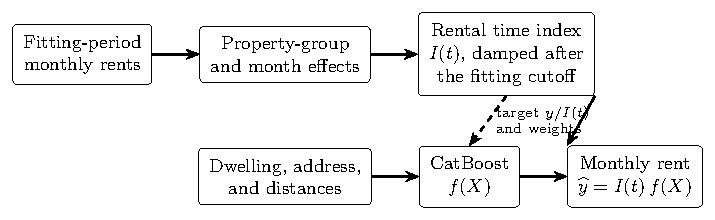
\includegraphics[width=0.96\linewidth]{model4_architecture.pdf}
\caption{Model~4: a global CatBoost with a property-adjusted
rental time index.
The dashed link supplies the index-normalized training target
and index-squared weights.
Predicted normalized rents are converted back to monthly rent
using the forecast index.}
\label{fig:model4-architecture}
\end{figure}

\textbf{Performance}

The fixed local control records Search RMSE 451.4529 and
Confirm RMSE 467.1128.
It uses a different MLP input configuration from Model~3's
448.24/462.87 run and is reported as a separate control,
rather than an exact reproduction of Model~3.

Table~\ref{tab:model4-trials} reports that control and the
successive configurations along the selected global-CatBoost
path.
The global direct-rent model reduces Search RMSE by 3.6776
and Confirm RMSE by 11.9000 relative to the local control.
Finer categorical target statistics, complete-address encoding,
and the rental time index then provide further reductions.

\begin{table}[htbp]
\centering
\caption{Fixed-split results in monthly-rent RMSE, SGD.
The local frozen control is a separate reference.
Each global-CatBoost row after the first retains the preceding
global configuration and adds the indicated modification.}
\label{tab:model4-trials}
\small
\setlength{\tabcolsep}{4pt}
\begin{tabularx}{\textwidth}{@{}Xrr@{}}
\toprule
Configuration & Search & Confirm \\
\midrule
Local frozen control
& 451.45 & 467.11 \\
\addlinespace
Global direct-rent CatBoost
& 447.78 & 455.21 \\
+ finer categorical statistics
& 445.38 & 452.87 \\
+ complete address
& 444.91 & 452.72 \\
\textbf{+ rental time index}
& \textbf{444.47} & \textbf{450.89} \\
\bottomrule
\end{tabularx}
\end{table}

The final model reduces RMSE relative to the fixed local
control by 6.9837 (1.55\%) on Search and 16.2182 (3.47\%)
on Confirm.
These are sequential experimental comparisons, not independent
causal ablations.

For context with Model~1, pooling Model~4's Search and Confirm
squared errors over October 2024--March 2025 gives
\[
\operatorname{RMSE}_{\mathrm{pooled}}
=
\sqrt{
\frac{
8{,}274\,\operatorname{RMSE}_{\mathrm{Search}}^2
+
8{,}924\,\operatorname{RMSE}_{\mathrm{Confirm}}^2
}{
17{,}198
}}
=
447.81.
\]
Model~1 reports RMSE 454.29 over the same calendar window.
The recorded difference is approximately 6.48 SGD, or 1.43\%.
The capacity-selection procedures differ: Model~4 uses
October--December 2024 for early stopping, so its pooled
score includes the period used to select its tree count.
This historical comparison does not establish an independent,
matched-protocol performance gain over Model~1.

A separate 50/50 blend of the global categorical-statistics
model and the local control achieved the lowest Search RMSE,
442.94.
Its Confirm RMSE was 454.37, compared with 452.87 for its
global component, and it was not retained.
This decision illustrates the use of Confirm in the iterative
development process.

Candidates failing their declared Search gates were not
evaluated on Confirm.
The vacancy correction failed during historical calibration,
before producing either score.
The final time-index candidate passed its Search threshold
of 444.9107 before one Confirm evaluation for that candidate.
Confirm had already been inspected in earlier trials, so
neither this gate nor the single candidate-level evaluation
makes Confirm an untouched test set.

The recorded competition submission used the frozen
fixed-split model to produce 50{,}000 predictions, without
refitting on all labelled rows.
The reported Kaggle RMSE is \textbf{441.46370}.
This is the latest submission already noted in the report.
The time-index model has the lowest Confirm RMSE among the
scored candidates in this series, but its Kaggle result does
not replace add\_mrt's 432.50 as the report's best competition
result.
Kaggle and local RMSEs evaluate different data.

Search and Confirm cover forecast months 1--6.
The original historical 16/22-month checks assessed the index
alone.
A separate rolling-origin study subsequently evaluated the
complete model recipe over 16 months at origins March 2022,
October 2022, and May 2023.
At each origin, the last three available history months select
a tree count; the index, preprocessing, and CatBoost are then
refitted through the origin before predicting the next
16 months without updating from their true rents.

That study records equal-origin RMSE 617.56, defined as the
square root of the mean origin MSE.
Its forecast windows differ from the fixed-split experiment,
and overlapping windows do not constitute independent market
cycles.
The results provide a separate assessment of the full model
over 16 months, while full-model evaluation across the entire
22-month competition horizon remains outstanding.

\subsection{Model 2: Auxiliary-feature CatBoost}\label{sec:m2}
We retain the tree family and compare locked feature configurations. The key question is whether additional location, transport and macro variables improve prediction beyond the original dwelling and address information. Development folds guide comparison; a longer 17-month assessment provides a distinct stress test. \textbf{MRT features are the most useful selected addition}: \texttt{add\_mrt} achieves development pooled RMSE 622.58 and 17-month RMSE \textbf{499.53}, versus 627.84 and 501.83 for original + address. Including all auxiliary families is worse (17-month RMSE 517.51 under cutoff-frozen macro and 553.50 under provided-lagged macro). The 17-month scores cannot be compared directly with Model~1's six-month scores; the fitting cutoffs differ.
\begin{table}[htbp]\centering\small
\caption{Locked auxiliary CatBoost comparisons. Dev. is pooled over three development folds; assessment is Nov 2023--Mar 2025. All values are RMSE (SGD).}\label{tab:auxmain}
\begin{tabular}{lrr}\toprule Configuration & Dev. pooled & 17-month\\\midrule
Original dwelling & 640.49 & 509.53\\
Original + address & 627.84 & 501.83\\
\textbf{Add MRT} & \textbf{622.58} & \textbf{499.53}\\
All auxiliary (cutoff-frozen) & 631.09 & 517.51\\
All auxiliary (provided-lagged) & 643.79 & 553.50\\\bottomrule\end{tabular}\end{table}


\paragraph{Why MRT, rather than all additional features?}
The add-MRT experiment improves pooled development RMSE by 5.26 SGD relative to the address baseline (627.84 to 622.58) and the longer assessment by 2.30 SGD (501.83 to 499.53). These are modest but consistent improvements on matched windows, unlike comparisons across independently chosen hold-outs. Distances and nearby-station counts supply accessibility detail not fully captured by the categorical address. The underlying rebuilt audit uses every supplied snapshot-open station entity for its open-distance pool, which may include LRT; this must not be confused with the narrower trunk-prefix definition in the separate 94-column multistage auxiliary table.

Broad addition is not a free improvement. The all-auxiliary CatBoost has a higher 17-month error under both macro timing choices. The cutoff-frozen setting holds the future macro vector to the preceding fit cutoff, while the provided-lagged setting assumes a completed prior month is already supplied. Even when that extra information is available, the larger feature set performs worse in the recorded experiment. Its behaviour could reflect redundancy, noise, estimation variance or interaction with the fixed tree configuration; the ablation does not establish a single causal explanation. Spatial coefficients and feature-family removal checks appear in Appendix~\ref{app:coremodels}.


\subsection{Model 3: Town-specific multistage model}\label{sec:m3}
This approach decomposes unit rent into a town-month trend and a flat-specific deviation. Town is used as the region because it balances geographic specificity and month-cell support (median 110.5 training flats per town-month; only 5.9\% of cells have fewer than 30). Each town has a three-layer, hidden-size-16 tanh RNN predicting mean \emph{rent per square metre} from the month index and previously available economic inputs. Within each town, a CatBoost and a five-dimensional full-covariance Gaussian mixture independently estimate the deviation from this mean. A shared MLP (128 and 64 hidden units, ReLU and 0.1 dropout) combines the estimated town mean, the two gaps, floor area and other unit attributes into final monthly rent. It does not multiply by floor area again after the MLP.

\begin{equation}\label{eq:stackmain}
\hat\mu_{c,t}=\mathrm{RNN}_c(t,\mathrm{lagged\ macro}),\qquad
\hat y_i=\mathrm{MLP}(\hat\mu_{c,t},\hat\delta^{\mathrm{CB}}_i,\hat\delta^{\mathrm{GMM}}_i,A_i,X_i).
\end{equation}
The RNN's weighted town-month unit-price RMSE is 0.9707 on validation and 1.0897 on test (SGD/m$^2$); this is \emph{not} the flat-level rent RMSE. After recombination, the independent CatBoost-gap and GMM-gap models reach validation rent RMSE 455.06 and 490.02, respectively. The shared stack reaches \textbf{448.24} validation RMSE and \textbf{462.87} on the untouched Jan--Mar 2025 test; epoch 8 is selected using validation only. Its reported training RMSE (461.25) uses in-sample town-CatBoost gap predictions, so that value is not a leakage-free out-of-fold stacking estimate. Architecture diagnostics are in Appendix~\ref{app:stack}.


\paragraph{Town trend versus individual deviation.}
Let $p_i=y_i/A_i$ denote rent per square metre for unit $i$ in town $c$ and approval month $t$. The multistage design treats the town-month mean $\mu_{c,t}$ as a shared component and $\delta_i=p_i-\mu_{c,t}$ as the within-town gap. The RNN estimates the former using time and earlier macro inputs, while two independently fitted gap models capture property-level heterogeneity. The CatBoost gap model can learn non-linear interactions and categorical splits; the Gaussian mixture supplies a separate distributional representation. Their predictions are combined only by the last shared MLP, rather than feeding one gap model's output into the other.

\begin{figure}[htbp]\centering
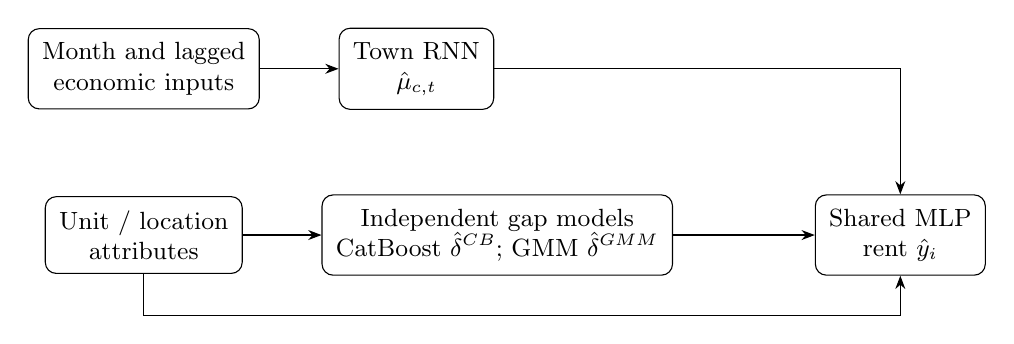
\begin{tikzpicture}[>=Stealth, every node/.style={font=\small},box/.style={draw,rounded corners,align=center,minimum height=0.67cm,inner sep=5pt},node distance=7mm and 10mm]
\node[box] (time) {Month and lagged\\economic inputs};
\node[box,right=of time] (rnn) {Town RNN\\$\hat\mu_{c,t}$};
\node[box,below=11mm of time] (unit) {Unit / location\\attributes};
\node[box,right=of unit] (gaps) {Independent gap models\\CatBoost $\hat\delta^{CB}$; GMM $\hat\delta^{GMM}$};
\node[box,right=18mm of gaps] (mlp) {Shared MLP\\rent $\hat y_i$};
\draw[->] (time)--(rnn);\draw[->] (unit)--(gaps);\draw[->] (gaps)--(mlp);\draw[->] (rnn.east) -| (mlp.north);\draw[->] (unit.south) |- ([yshift=-5mm]mlp.south) -- (mlp.south);
\end{tikzpicture}
\caption{Multistage inference: the two gap estimates are independent inputs to a shared final rent regressor.}\label{fig:stackdiagram}
\end{figure}

This architecture was motivated by the possibility that a town-specific rental path is easier to learn than an absolute rent for every type of flat. The town granularity has enough observations in most training month-cells to estimate such paths, while finer block-month partitions would be sparse. The RNN is not autoregressively fed the true previous rent; it carries the sequence of previously known economic features in its hidden state. Its unit-price RMSE is deliberately presented separately from SGD rent RMSE, since the two target definitions differ. A direct multiplication of the predicted unit price by area is not the final architecture: area and the predicted mean and gaps enter the shared MLP, allowing it to learn that conversion alongside other attributes.

The final validation gain is also interpretable as a model-combination test. Using the CatBoost gap alone gives 455.06 SGD validation RMSE, the Gaussian-mixture gap alone 490.02, and their shared MLP 448.24. The improvement over CatBoost alone is 6.82 SGD. The reported 462.87 test RMSE follows selection of epoch 8 on validation alone. However, the in-sample CatBoost-gap training predictions were not rebuilt as out-of-fold inputs; this is an important limitation for a clean stacking interpretation.


\subsection{Model 4: Global CatBoost with adjusted rental time index}\label{sec:m4}
A pooled CatBoost addresses time extrapolation without training separate town models. It takes 26 inputs (17 numeric and 9 categorical), including complete address, property characteristics, geographic distances and approval time. A property-adjusted index is estimated \emph{only on fitting-period rents} by the fixed-effects model
\begin{equation}\label{eq:indexmain}
\log y_i=\alpha_{g(i)}+b_{t(i)}+\epsilon_i,\qquad
I(t)=\exp(b_t-b_T),\quad T=\text{Sep 2024}.
\end{equation}
For months after cutoff, the final six fitted month effects determine a slope $s$ damped by $\phi=0.9$: $\hat b_{T+h}=b_T+s\phi(1-\phi^h)/(1-\phi)$. CatBoost learns $z_i=y_i/I(t_i)$ with index-squared weights; predictions return to SGD as $\hat y_i=I(t_i)f(X_i)$. The retained model has 496 trees (depth 8, learning rate 0.05). The final sequential configuration reaches Search RMSE \textbf{444.47} and Confirm RMSE \textbf{450.89}, against 447.78 and 455.21 for its global baseline. Its frozen competition submission scores \textbf{441.46}. Confirm was consulted in iterative development, so it is not claimed as an untouched test. Further ablations and alternative local-history experiments are in Appendix~\ref{app:time}.


\paragraph{Training and inference of the rental index.}
The adjusted time-index model differs from predicting the raw month number directly. It first fits month fixed effects jointly with property-group effects to separate changes in the composition of observed flats from a shared rental-level shift. Group effects control for persistent differences between property groups; the exponentiated month-effect difference forms a multiplicative rent index anchored at September 2024. Applying its inverse to observed rent gives the response on which the pooled CatBoost is trained. Predictions are subsequently multiplied by the forecast index to restore the target scale.

Because post-cutoff month fixed effects are not known, the source extrapolates from the final six training-month effects and damps the estimated monthly slope with $\phi=0.9$. The index is therefore a forecast assumption rather than a directly observed future label statistic. Index-squared sample weights correspond to treating errors in the normalized target so that errors after rescaling matter in nominal rent. In the reported sequential configuration, the Search RMSE improves by 3.31 SGD (447.78 to 444.47) and Confirm by 4.32 SGD (455.21 to 450.89) relative to its matched global CatBoost baseline. The result is stronger evidence about this specific correction than a comparison with Models~1--3, whose fitting configurations and evaluation windows differ.

\subsection{Model 5: Temporal and Historical CatBoost}

Our approach extends CatBoost with temporal modelling and historical rental features. Unlike the auxiliary-feature CatBoost experiments, this model uses an independent feature pipeline, with particular emphasis on market changes and previous transactions from the same HDB block.

\paragraph{Preprocessing and Base Model.}
We constructed 34 baseline features from property attributes, rental dates and geographical information. These include categorical variables such as town, block, street and flat type, together with numerical features describing building characteristics and proximity to MRT stations, schools and shopping malls.

The main experiments used CatBoost with depth 6, learning rate 0.055, L2 regularisation 5 and random seed 42. We used chronological validation rather than random splitting to reflect the forward prediction task.

\paragraph{Temporal Modelling.}
The baseline already included calendar and continuous time features. We further introduced cyclical month features,
\[
m_{\sin}=\sin\left(\frac{2\pi(m-1)}{12}\right),
\qquad
m_{\cos}=\cos\left(\frac{2\pi(m-1)}{12}\right),
\]
and a composition-adjusted rental market index estimated from historical log rents across town and flat-type groups. Recent market changes were extrapolated with exponential decay to limit long-term trend growth.

The final prediction applies a multiplicative correction:
\begin{equation}
\hat{y}_{i,t}
=
f_{\mathrm{CB}}(x_{i,t})
\exp(\alpha\Delta_t),
\end{equation}
where $\Delta_t$ represents the estimated market-index change and $\alpha=0.5$ controls the correction strength. Forward corrections are applied only beyond the training cutoff.

\paragraph{Chronological Validation.}
We used three six-month development periods: July--December 2023, January--June 2024 and July--December 2024. Each model was trained only on data preceding its validation period. January--March 2025 was evaluated separately as a diagnostic period. The reported development RMSE is the arithmetic mean of the three fold-level RMSE values.

\paragraph{Temporal Ablation.}
We compared the original model (A), additional seasonality (B), market trend correction (C), and both components (D), keeping the CatBoost configuration fixed.

\begin{table}[t]
\centering
\caption{Temporal ablation at 1600 iterations (RMSE).}
\label{tab:f1_temporal}
\small
\begin{tabular}{lcc}
\hline
Model & Dev. mean & 2025 Q1 \\
\hline
A: Baseline & 519.60 & 450.39 \\
B: + Seasonality & 519.48 & 450.38 \\
C: + Market trend & 518.41 & 449.87 \\
D: + Both & \textbf{517.89} & \textbf{449.80} \\
\hline
\end{tabular}
\end{table}

The market correction produced a larger improvement than seasonality alone. Combining both features reduced the development RMSE from 519.60 to 517.89.

We also evaluated different boosting iterations while keeping other hyperparameters unchanged.

\begin{table}[t]
\centering
\caption{Development RMSE across boosting iterations.}
\label{tab:f1_iterations}
\small
\begin{tabular}{rcc}
\hline
Iterations & Model A & Model D \\
\hline
800  & 520.17 & 518.51 \\
1200 & \textbf{519.60} & 517.95 \\
1600 & 519.60 & 517.89 \\
2000 & 519.74 & \textbf{517.88} \\
\hline
\end{tabular}
\end{table}

For Model D, increasing from 1600 to 2000 iterations improved mean RMSE by only 0.01. The 1600-iteration configuration also performed slightly better in our separate long-horizon evaluation and was therefore selected for subsequent experiments.

\paragraph{Historical Rental Features.}
We next investigated whether previous transactions from the same block could improve predictions beyond existing location features.

For each observation, we identified earlier rentals sharing the same town, block, street and flat type. Five features were constructed: transaction count, median rent, mean rent, standard deviation and months since the most recent transaction.

To prevent target leakage, only transactions from strictly earlier months were included. Validation features used only labels available before the corresponding training cutoff; same-month and validation-period labels were excluded.

We compared five configurations:
\begin{itemize}
    \setlength{\itemsep}{0pt}
    \item F0: Temporal model D.
    \item F1: F0 with block-level rental history.
    \item F2: F1 with street- and town-level history.
    \item F3: F2 with recent 3/6/12-month rental statistics.
    \item F4: F3 with nearby comparable rentals.
\end{itemize}

\begin{table}[t]
\centering
\caption{Historical rental feature ablation (RMSE).}
\label{tab:f1_history}
\small
\begin{tabular}{lcc}
\hline
Model & Dev. mean & 2025 Q1 \\
\hline
F0: Temporal baseline & 517.89 & 449.80 \\
F1: + Block history & \textbf{514.83} & \textbf{444.29} \\
F2: + Street/Town history & 519.01 & 445.80 \\
F3: + Recent windows & 528.70 & 445.44 \\
F4: + Nearby rentals & 535.78 & 445.63 \\
\hline
\end{tabular}
\end{table}

F1 achieved the lowest development RMSE, improving over F0 by 3.07 SGD. Its 2025 Q1 diagnostic RMSE also decreased from 449.80 to 444.29.

Adding more historical features did not consistently help. In particular, recent-window features became less reliable over longer prediction horizons because no new labelled rentals were available after the training cutoff. We further tested four enhanced configurations (G1--G4), including time-normalised rents and cutoff-anchored windows, but none improved upon F1's development RMSE of 514.83.

\paragraph{Kaggle Evaluation.}
After model selection, we retrained the final configuration on all 150,000 labelled records and generated predictions for 50,000 test samples.

\begin{table}[t]
\centering
\caption{Kaggle Public Leaderboard RMSE.}
\label{tab:f1_kaggle}
\small
\begin{tabular}{lc}
\hline
Submission & RMSE \\
\hline
Initial CatBoost & 441.78158 \\
D1200: Temporal model & 439.55517 \\
D1600: Temporal model & 438.28697 \\
F1 1600: + Block history & \textbf{432.50394} \\
\hline
\end{tabular}
\end{table}

The final F1 model achieved a Public Leaderboard RMSE of 432.50394, improving upon D1600 by 5.78 SGD and the initial submission by 9.28 SGD (2.10\%). This improvement is consistent with the chronological validation results and demonstrates the usefulness of block-level rental history.

\paragraph{Discussion and Limitations.}
Our experiments suggest that local historical rental information is more effective than simply increasing model complexity or adding broader historical statistics. However, sparse block histories and changing market conditions can reduce reliability over longer forecast horizons. Repeated Public Leaderboard evaluation also introduces a risk of overfitting model selection to the public test subset. These limitations motivate more robust, temporally consistent history features and evaluation on independent future periods.

\begin{table}[htbp]\centering\small
\caption{Matched local experiment for the global CatBoost index. All metrics are monthly-rent RMSE (SGD).}\label{tab:indexablation}
\begin{tabular}{lrr}\toprule Configuration & Search: Oct--Dec 2024 & Confirm: Jan--Mar 2025\\\midrule
Global CatBoost baseline & 447.78 & 455.21\\
With rental time index & \textbf{444.47} & \textbf{450.89}\\\bottomrule\end{tabular}\end{table}

The index model is particularly relevant when the market is not stationary: it makes extrapolation an explicit component rather than asking a tree to extrapolate beyond the largest observed month index. Its accuracy still depends on the assumption that recent adjusted month effects describe the future trajectory. The Confirm window was examined during iteration, so the comparison is useful but should not be represented as a pristine, independently held-out model-selection test.


\section{Comparison and discussion}\label{sec:discussion}
\begin{table}[htbp]\centering\small
\caption{Headline scores (SGD RMSE). Different rows evaluate different data and must not be used as a direct model leaderboard.}\label{tab:headline}
\begin{tabularx}{\linewidth}{@{}Xl r@{}}\toprule
Model & Evaluation & RMSE\\\midrule
Core CatBoost & Six-month hold-out & 454.29\\
Auxiliary \texttt{add\_mrt} & 17-month assessment & 499.53\\
Multistage & Validation / test & 448.24 / 462.87\\
Global CatBoost + index & Search / Confirm & 444.47 / 450.89\\
Best competition submission (\texttt{add\_mrt}) & Competition & \textbf{432.50}\\
Latest submission (global + index) & Competition & 441.46\\\bottomrule
\end{tabularx}\end{table}

The selected MRT features improve over a matched address-only auxiliary baseline, whereas adding all available families hurts long-window CatBoost performance. The multistage method improves over its individual gap components but requires multiple town-specific stages. Global time-index modelling improves a fixed local baseline, though its extrapolation beyond the six locally scored months is only partly checked. An additional reported local block-history variant (\texttt{F1}, 1,600 trees) also reaches a Kaggle \emph{public leaderboard} RMSE of 432.50394; that result is retained separately in Appendix~\ref{app:time}, since the source identifies it by its own leaderboard setting and label, not by the locked \texttt{add\_mrt} experiment. Public leaderboard and competition/private-test terminology should not be conflated without confirmation.

\textbf{Limitations.} Historical target encodings depend on prior available labels and can become sparse at long horizons; MRT/school/mall snapshots lack complete opening histories; straight-line distance is not walking time; and spatial relationships are predictive associations, not causal premiums. Some multistage training features were produced by in-sample models. Repeated leaderboard checks can overfit to the competition split. Most importantly, unlike a matched-split ablation, the different local windows in Table~\ref{tab:headline} cannot establish that one algorithm universally outperforms the others.


\subsection{What the experiments establish}
Three lessons emerge from comparisons within the same evaluation design. First, modelling individual dwelling, location and time interactions improves markedly over nested historical means; the six-month baseline drops from 565.58 to 454.29 RMSE when moving from town-plus-flat-type means to CatBoost. Second, selective spatial enrichment matters: adding MRT features to an address baseline improves both development and assessment results, but including all available auxiliary families does not. Third, explicit treatments of temporal and local variation can be effective: the multistage combination improves validation RMSE over either individual gap component, and the adjusted time index improves over its own global CatBoost control on both Search and Confirm.

The experiment-level conclusions are more defensible than a cross-window ranking. Auxiliary CatBoost's 499.53 is measured over 17 months using a fit ending October 2023, while the 454.29 core score evaluates six months using data through September 2024. The multistage validation/test and global Search/Confirm use a recent split but different selection processes. Accordingly, the performance table is an account of outcomes rather than a controlled head-to-head between all four architectures.

\subsection{Reproducibility and remaining risks}
The primary controls are row-order preservation, date parsing shared by labelled and unlabelled datasets, training-only target-dependent feature construction, explicit fitting cutoffs, and fixed comparison configurations. These prevent a useful-looking auxiliary feature from quietly importing the future rental outcome. Remaining risks include unavailable unit-floor and renovation information, spatial snapshot timing, sparse historical labels in the 2025--2026 private period, and public leaderboard selection effects. A next evaluation should use a single later chronological hold-out for all candidate pipelines, out-of-fold gap training for the multistage model, and feature-availability simulations matching the unlabelled competition horizon. Those checks would be needed before claiming superiority beyond the observed experiments.



\subsection{Error patterns and model choice}
The core error breakdown further clarifies what the headline RMSE conceals. Across October 2024--March 2025, monthly six-month hold-out RMSE ranges from 438.22 to 471.08 SGD; corresponding mean errors are negative in every month. The monthly variation in RMSE is much smaller than the mean-error drift seen in the oldest rolling folds, so the central difficulty is not just fitting a complex cross-sectional mapping. The model also needs to represent changes in the overall rent level. This is why the multistage approach isolates a shared town-month movement and the global time-index approach explicitly estimates a market factor.

Differences between flat categories suggest a second difficulty. On the core six-month hold-out, executive flats have RMSE 537.59 across 852 scored rows, compared with 471.58 for 5-room flats (3,908 rows) and 426.74 for 3-room flats (5,687 rows). Only seven 1-room flats appear in this scored period, so their 461.55 RMSE is too unstable to draw a reliable subtype conclusion. Larger error for the executive category need not imply that the flat-type encoding is inadequate: floor position, renovation and tenant-specific conditions are not observed. These examples justify reporting group-level error alongside aggregate RMSE, while leaving the full diagnostic tables in Appendix~\ref{app:coremodels}.

\subsection{Feature importance versus measured improvement}
The preliminary core CatBoost attributes the largest importance to flat type, month index and town. That is a property of a particular fitted tree and its correlated inputs, not evidence of a causal rent premium. In contrast, the locked auxiliary comparison is an empirical test of a feature family: the difference between original+address and add-MRT is measured with the same cutoffs and metric. We therefore use the matched experiment to judge whether a new feature family helps, and use importance only to explain which fields the fitted baseline relies upon. For example, a station-distance association cannot establish how much rent would change if a station were built, and an index trend cannot prove the source of a macroeconomic price movement.

\subsection{How a final prediction is produced}
The four pipelines have different serving-time requirements. Core CatBoost needs standardized original rental descriptors and the derived date/lease information. Auxiliary CatBoost additionally joins a block to its known coordinates and station features, then applies the locked tree. The multistage model evaluates a town-specific trend and two independent within-town gap estimators before combining their outputs in the global MLP. The global index model estimates the projected month index and rescales a normalized CatBoost prediction. Although the methods can be compared on their recorded local experiments, they are not freely interchangeable at inference time: historical rent encodings and external time series must be available for the scored month under the same assumptions used in validation.

The best private competition result, 432.50 RMSE, is associated with the add-MRT configuration in the saved report, while the more recent global-index submission scores 441.46. Both are reported as observed submission outcomes; neither should be retroactively used to select a model on the nominally held-out local test period. The public-leaderboard F1 result discussed in Appendix~\ref{app:time} has a numerically similar score but originates from a separately labelled historical-feature experiment. Keeping those provenance labels intact avoids inventing equivalences between experimental runs.


\subsection{Evaluation design: sources of uncertainty}
Chronological validation controls one important source of optimistic bias: a rental approved in 2025 should not influence the training of a model meant to predict 2024. It does not, however, automatically prevent every type of look-ahead. A station labelled ``open'' in a snapshot may not have been open in an earlier approval year; the auxiliary sources do not provide the opening dates needed to reconstruct the precise historical transport network. Similarly, same-month macro observations are not valid predictors if they would only become available after approval. We therefore separate geometric snapshot features, completed-month macro lag features, and genuinely label-derived histories in the modelling narrative.

The scored interval also changes the question being answered. The core six-month evaluation has 17,198 scored rows and directly measures short-range extrapolation from September 2024. The 17-month auxiliary assessment is harder to interpret as a matched comparison with that core score, because it trains only through October 2023. Its purpose is to challenge the locked feature variants over a longer horizon. The sequential Search/Confirm experiment and multistage validation/test each divide the six latest labelled months into two subperiods, but their selection procedures differ. In particular, the global model's Confirm period was consulted in its optimization series, whereas the multistage test is described as scored after its validation-based choice. We report that distinction even when both groups of results look close in numerical RMSE.

\subsection{Quantitative contribution of the strongest changes}
\begin{table}[htbp]\centering\small
\caption{Improvements within matched experiments. A positive difference means lower RMSE (SGD); comparisons are not pooled across rows.}\label{tab:deltas}
\begin{tabularx}{\linewidth}{@{}Xlrr@{}}\toprule
Comparison & Same scoring window & Earlier & Improved\\\midrule
Town+flat-type mean $\rightarrow$ core CatBoost & Six-month hold-out & 565.58 & 454.29\\
Address baseline $\rightarrow$ add-MRT & Development pooled & 627.84 & 622.58\\
Address baseline $\rightarrow$ add-MRT & 17-month assessment & 501.83 & 499.53\\
Single CatBoost gap $\rightarrow$ multistage MLP & Multistage validation & 455.06 & 448.24\\
Global baseline $\rightarrow$ time index & Search & 447.78 & 444.47\\
Global baseline $\rightarrow$ time index & Confirm & 455.21 & 450.89\\\bottomrule
\end{tabularx}\end{table}

The largest measured change in this table comes from moving beyond a simple town-by-type average: more detailed property variables and nonlinear splits are essential. Later innovations are smaller and more targeted. MRT is a modest but robust auxiliary increment in its particular locked comparisons. Combining the independent gap estimates is helpful for the validation-period multistage architecture, though proper out-of-fold training of the stack would improve its methodological cleanliness. The rental index makes a consistent local improvement within a single global model family, but its effect relies on the estimated future trend. These statements remain limited to the evaluation windows and input availability actually used by each experiment.

\subsection{Scope of the retained and removed material}
We retain the preprocessing rules that materially affect prediction and submission correctness, the splits and target definitions needed to interpret performance, the core and auxiliary ablation results, and enough architecture detail to distinguish each modelling approach. Full inventories of postal, station, school, mall, COE and stock descriptors are moved to the appendix because they are largely a search space, not the winning model's final feature list. The appendix preserves compact EDA findings, cleaning audits, feature availability rules and extended component trials, while omitting most exploratory figures. This allows a reader to reproduce or audit the feature choices without forcing every exploratory branch into the main technical argument.

\section{Conclusion}\label{sec:conclusion}
Careful chronological validation and selective feature engineering matter more than maximizing feature count. Core CatBoost provides a strong 454.29 six-month hold-out baseline. Of the tested auxiliary groups, MRT yields the best locked CatBoost development result, while the multistage and global time-index approaches demonstrate different ways to handle regional and temporal effects. The best reported competition RMSE is \textbf{432.50} (\texttt{add\_mrt}); the latest separate submission scores 441.46. Gold Miner (Group 12) is reported at rank 21 after eight submissions. Appendix material preserves the extended exploratory analysis, unused feature definitions and secondary experiments without expanding the main narrative.

\clearpage
\appendix
\section{Supplementary exploratory data analysis}\label{app:eda}
The labelled file contains 150,000 rows over 51 approval months (Jan 2021--Mar 2025); the unlabelled competition file contains 50,000 rows over 17 months (Mar 2025--Jul 2026). Both have ten input columns and no missing cells. Approval-date notation differs (\texttt{March-25} versus \texttt{2025-03}) and is standardized before feature creation. The unlabelled file overlaps the labelled data in \emph{calendar month}, not in labels or row identities.

\begin{table}[htbp]\centering\small
\caption{Selected EDA findings and their modelling implications.}\label{tab:eda-summary}
\begin{tabularx}{\linewidth}{@{}p{0.31\linewidth}X@{}}\toprule
Observation & Implication \\\midrule
Town--flat-type medians & Among cells with at least 200 records, medians range from SGD 2,000 (Bukit Merah, 2-room, $n=303$) to SGD 4,650 (Central, 5-room, $n=200$). Location and flat type should interact.\\
Monthly rental trend & Raw medians and composition-adjusted descriptive ridge residuals differ across months; approval time cannot be ignored. The ridge is fitted to all labelled months, so it is \emph{not} an out-of-sample evaluation.\\
Geographical distribution & 8,134 blocks have at least five rentals; spatial summaries suggest local variation beyond the town label.\\
Dwelling composition & Floor area, flat model, and lease-age distributions vary by flat type and place; descriptive differences must not be interpreted as causal effects.\\\bottomrule
\end{tabularx}\end{table}
These checks motivate the selected models, but the full descriptive map panels, masked low-count cells, and unadjusted rental distributions are omitted to prioritize predictive evidence. No input rows are discarded on the basis of EDA alone.

\section{Core cleaning and excluded fields}\label{app:core}
\begin{table}[htbp]\centering\small
\caption{Deterministic cleaning and unlabelled coverage audit.}\label{tab:clean-compact}
\begin{tabular}{lrrl}\toprule
Field & Labelled levels before & After & Important note \\\midrule
Street & 1,146 & 576 & 30,781 labelled rows normalized\\
Flat type & 11 & 6 & 35,331 rows standardized\\
Town & 26 & 26 & No unseen unlabelled town\\
Flat model & 20 & 20 & No unseen unlabelled flat model\\
Block & 2,720 & 2,720 & 11 unseen block labels (36 rows)\\
Building & 9,406 & 9,406 & 50 unseen buildings (102 rows)\\\bottomrule
\end{tabular}\end{table}
Street normalization changes 10,482 unlabelled rows. A building is \texttt{normalized block + normalized street}; using block number alone would confuse addresses. Approval dates are parsed into year, calendar month and index $12(y-2021)+(m-1)$; labelled indices span 0--50 and unlabelled indices extend to 66. Lease age is approval year minus lease commencement year. One reversed-year record is retained with derived lease age set missing and an invalid-age flag. All original rental records, duplicate-like observations and unusual rents remain; competition row order is preserved.

Furnished status (always \texttt{yes}) and upfront fee (always zero) have no predictive variation and are removed from the core baseline. For the multistage model, flat-type rank (1-room--5-room, executive) and a fixed flat-model rank are added, while normalized categorical identifiers remain available to the trees. Numeric imputations, standardizations and target-dependent encodings are fitted separately within each model's training window. These rules avoid applying fitted statistics from scored months to the training pipeline.

\section{Auxiliary inventory and feature availability}\label{app:aux}
The rebuilt audit investigated 1,878 conceptual feature candidates, of which 1,595 are month-panel candidates; a separate 94-column auxiliary table was supplied to the multistage model. These are distinct inventories rather than the number of features in any fitted CatBoost model.
\begin{table}[htbp]\centering\small
\caption{Candidate inventory; counts refer to audit features, not a final model.}\label{tab:feature-families-short}
\begin{tabular}{lr@{\qquad}lr}\toprule Family & Count & Family & Count\\\midrule
Block structure & 5 & Location & 11\\
MRT & 122 & Schools & 123\\
Malls & 8 & COE & 164\\
Stocks & 1,200 & Adjusted-price sensitivity & 231\\
Original / derived & 14 & Total & 1,878\\\bottomrule\end{tabular}\end{table}

\textbf{Block and proximity.} The block--street join is one-to-one at rental-row level and supplies latitude, longitude, planning region, year completed and maximum block floor. The maximum floor is \emph{not} the individual unit's floor. Distances use a great-circle formula (Earth radius 6,371 km); their measured straight-line distance is not travel time. Features include CBD distance, nearby-block counts, nearest MRT/school/mall distances and selected counts within radii. Source inventories include 337 schools and 113 malls. The original trunk MRT feature set considers open prefixes NS, NE, CC, DT, TE, EW and CG separately from future-line prefixes; the rebuilt add-MRT experiment uses the broader snapshot-open station pool, potentially including LRT. The two definitions should not be silently combined.

\textbf{Temporal variables.} Each rental in month $T$ receives COE and equity information from the previous completed month $T-1$, with a small number of multi-month COE summaries. There are 77 audited equity symbols. The bank basket uses \texttt{D05.SI}, \texttt{O39.SI}, \texttt{U11.SI}; the property basket uses \texttt{C09.SI}, \texttt{U14.SI}, \texttt{9CI.SI}. Missing early constituent data are left missing. COE bidding rounds use round 2 where present, otherwise round 1. These market observations are shared by flats in the same approval month, not independent flat-level measurements.

\textbf{Recent-rent features.} Six smoothed three-month preceding-label group means are available for postal sector, district, nearest mall, nearest open MRT station, nearest primary school and nearest secondary school, with shrinkage strength 20 (Equation~\eqref{eq:shrinkmain}). At the start of labelled history, such means are unavailable. In the distant unlabelled months they cannot be refreshed using unknown private labels.

\textbf{Limitations and excluded detail.} The facility snapshots lack reliable opening dates; some MRT coordinate precision is limited; 159 labelled rows have block floor/completion sentinels; 285 blocks have missing postal codes; and schools/malls are static snapshots. Full stock-level feature columns, adjusted-close sensitivity variations and map-level target-mean visualizations are excluded from this concise appendix because they do not establish a reproducible improvement in the chosen model. Importantly, the fixed auxiliary comparison reports that adding all candidate feature families \emph{worsens} the 17-month RMSE relative to add-MRT.

\section{Additional CatBoost diagnostics}\label{app:coremodels}
The core CatBoost uses depth 8, learning rate 0.05, 600 iterations and seed 42; native categorical inputs contain the cleaned property and address fields. Mean baselines use only fitting-period labels. The six-month hold-out is Oct 2024--Mar 2025 after a fit through Sep 2024.
\begin{table}[htbp]\centering\small
\caption{Core CatBoost rolling one-year folds; mean error is predicted minus actual SGD.}\label{tab:rolling-short}
\begin{tabular}{lrrr}\toprule Scored year & Fit rows & RMSE & Mean error\\\midrule
Apr 2022--Mar 2023 & 46,756 & 719.52 & $-370.41$\\
Apr 2023--Mar 2024 & 78,960 & 599.59 & $-146.57$\\
Apr 2024--Mar 2025 & 114,842 & 477.47 & $-35.74$\\\bottomrule\end{tabular}\end{table}
\begin{table}[htbp]\centering\small
\caption{Monthly errors on the six-month core hold-out (SGD).}\label{tab:monthly-short}
\begin{tabular}{lrrr}\toprule Month & RMSE & MAE & Mean error\\\midrule
Oct 2024 & 438.22 & 326.54 & $-35.05$\\
Nov 2024 & 464.91 & 330.08 & $-22.80$\\
Dec 2024 & 447.66 & 325.29 & $-18.14$\\
Jan 2025 & 471.08 & 346.60 & $-37.51$\\
Feb 2025 & 453.18 & 338.46 & $-48.63$\\
Mar 2025 & 449.69 & 332.37 & $-53.33$\\\bottomrule\end{tabular}\end{table}
The chronological hold-out scores 454.29 versus 476.25 for a same-sized random hold-out. Mean errors are $-36.29$ and $-6.64$, respectively. Adding calendar-month sine and cosine to the existing year/month/index fields increases rolling-fold RMSE from 719.52 to 729.00, 599.59 to 610.34, and 477.47 to 477.83; hence the cyclical pair was not retained. Executive flats ($n=852$) have 537.59 RMSE, while 5-room ($n=3,908$) and 3-room ($n=5,687$) flats have 471.58 and 426.74 RMSE. The 1-room category has only seven scored observations and is too small for a strong conclusion.

\textbf{Auxiliary diagnostics.} The rebuilt feature-family study uses three expanding development folds (May--Oct 2022, Nov 2022--Apr 2023, May--Oct 2023) and a separate 17-month Nov 2023--Mar 2025 assessment after fitting through Oct 2023. All main CatBoost configurations use locked hyperparameters. Cutoff-frozen macro holds the vector fixed at the fitting cutoff, while provided-lagged uses the preceding completed month of each rental. Under cutoff-frozen timing, 17-month RMSE is 509.53 (original dwelling), 501.83 (original+address), 499.53 (add-MRT), and 517.51 (all main auxiliary). Under provided-lagged timing, the all-main-auxiliary score is worse at 553.50. The MRT improvement is small but consistent within its matched evaluation design; the much earlier training cutoff makes comparison with the six-month core score invalid.

\section{Multistage implementation details}\label{app:stack}
For rent per square metre $p_i=y_i/A_i$, the training town--month aggregate is $\mu_{c,t}=\mathrm{mean}_{i\in(c,t)}p_i$. Individual deviation is $\delta_i=p_i-\mu_{c,t}$. Each town uses a recurrent network for the sequence of its monthly means and two \emph{independent} predictors for the within-town deviation. The shared MLP receives their outputs along with floor area, time and property attributes, then predicts SGD monthly rent.

\begin{table}[htbp]\centering\small
\caption{Selected multistage local metrics; units differ by target.}\label{tab:stack-short}
\begin{tabularx}{\linewidth}{@{}Xrr@{}}\toprule Component / metric & Validation & Test\\\midrule
Three-layer town RNN, unit-price cell RMSE (SGD/m$^2$) & 0.9707 & 1.0897\\
Linear-bypass town model, unit-price cell RMSE (SGD/m$^2$) & 1.9646 & 3.4044\\
CatBoost-gap, final rent RMSE (SGD) & 455.06 & --\\
Gaussian-mixture-gap, final rent RMSE (SGD) & 490.02 & --\\
Shared MLP, final rent RMSE (SGD) & \textbf{448.24} & \textbf{462.87}\\\bottomrule\end{tabularx}\end{table}

\textbf{Training choices.} The town RNN is fit for 50 epochs (learning rate 0.01, seed 5228). The town CatBoost gap estimators use depth 8, learning rate 0.05, up to 1,000 iterations, validation early stopping (patience 50), median imputation of numeric columns and native categories. Inputs cover coordinates, block/street, flat type/model, nearest transport and amenity descriptors. A town-specific Gaussian mixture starts at 20 components and reduces its count until each hard-assigned training component has at least 30 rows; accepted component counts range from 3 to 19. The shared MLP uses 27 numeric features, Adam (learning rate 0.001) and batch size 1,024. Epoch 8 is selected using validation only. Component training predictions for the CatBoost gap are in-sample rather than cross-fitted, so the stack training RMSE of 461.25 should not be read as unbiased training-stage generalization evidence.

\textbf{Separate exploratory trials.} Earlier dollar-denominated town-month forecasts are not the chosen unit-price network. A one-layer dollar RNN achieved validation/test \emph{cell} RMSE 93.25/88.04, and a four-input three-layer LSTM 88.75/83.39. A linear-bypass dollar model deteriorated to 170.56/261.29. These cell scores are not flat-level prediction RMSEs and did not select the final multistage stack. A separate column-ablation procedure screened one auxiliary column at a time against the current saved feature set, retained candidate groups only when validation improved, and stopped when no candidate group won; its selection was distinct from the locked CatBoost feature-family comparisons.

\section{Global index and local history experiments}\label{app:time}
The global index model fits $\log y_i=\alpha_{g(i)}+b_{t(i)}+\epsilon_i$ on training data and forecasts the post-cutoff index from recent adjusted month effects. It predicts normalized rental $y/I(t)$ with an otherwise shared CatBoost configuration (496 trees, depth 8, learning rate 0.05) and converts back to SGD. The extrapolation slope is damped by $\phi=0.9$. It improves its matched Search/Confirm baseline RMSE from 447.78/455.21 to 444.47/450.89; its recorded competition score is 441.46. The Confirm period was inspected during development and should not be called untouched.

A separate historical-rent CatBoost series explores calendar seasonality, time trend adjustments and prior block rentals. It uses 1,600 boosting iterations in its main ablation. Adding historical rent summaries at the block level (\texttt{F1}) reduces the series' mean local RMSE from 517.90 (temporal-only \texttt{F0}) to 514.83. On the first quarter of 2025, the change is 449.80 to 444.29. Its recorded \emph{public leaderboard} score is 432.50394, versus 438.28697 for the temporal-only submission; these are separate from the locked add-MRT experiment even though one displayed score rounds to the same two decimals. Another version with fixed cutoff histories and normalized statistics did not consistently improve on F1 (mean local RMSE 515.01--517.35).

\textbf{Interpretation.} Across the retained experiments, the most convincing gains arise from matched ablations: add-MRT versus original+address, shared multistage MLP versus its component-only rent estimators, the adjusted index versus the same global CatBoost, and block-history F1 versus its temporal-only predecessor. The remaining methodological limitation is heterogeneous cutoffs and possible imperfect inference-time history availability. A strict head-to-head comparison would retrain all finalists on the same cutoff and evaluate the same later months without consulting that period during selection.
\end{document}
